\documentclass[crop, tikz]{standalone}
\usepackage{tikz}
\usepackage{pgfplots}

\begin{document}
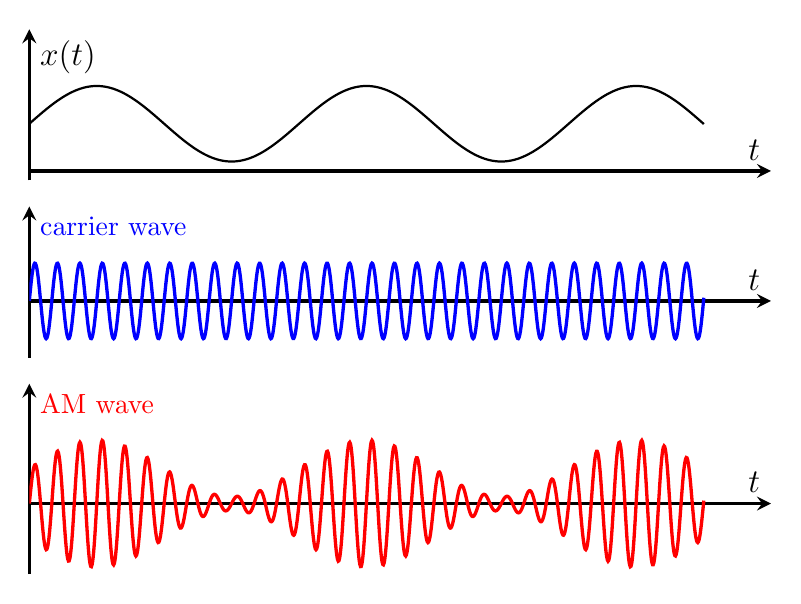
\begin{tikzpicture}[samples=1000, domain=0:10*pi]

	\begin{axis}[
		width=11cm, height=3.5cm,
		xtick=\empty,
		ytick=\empty,
		xlabel={\large $t$},
		ylabel={\large $x(t)$},
		xmin=0, xmax=11*pi,
		ymin=-0.5, ymax=7.5,
		axis lines = middle,
		very thick,
		trig format = rad
	]
		\addplot [no markers, smooth, thick] {2.5 + 2*sin(0.5*x)};
	\end{axis}
		
	\begin{axis}[
		at={(0, -2.25cm)},
		width=11cm, height=3.5cm,
		xtick=\empty,
		ytick=\empty,
		xlabel={\large $t$},
		ylabel={\textcolor{blue}{carrier wave}},
		xmin=0, xmax=11*pi,
		ymin=-3, ymax=5,
		axis lines = middle,
		very thick,
		trig format = rad
	]
		\addplot [no markers, smooth, blue, very thick] {2*sin(6*x)};
	\end{axis}
		
	\begin{axis}[
		at={(0, -5cm)},
		width=11cm, height=4cm,
		xtick=\empty,
		ytick=\empty,
		xlabel={\large $t$},
		ylabel={\textcolor{red}{AM wave}},
		xmin=0, xmax=11*pi,
		ymin=-10, ymax=17,
		axis lines = middle,
		very thick,
		trig format = rad
	]
		\addplot [no markers, smooth, red, very thick] {(2.5 + 2*sin(0.5*x)) * 2*sin(6*x)};
	\end{axis}
\end{tikzpicture}
\end{document}
